% Define block styles
\tikzstyle{blockS} = [text centered, text width=1.2cm, minimum height=0.5cm, rounded corners=true]
\tikzstyle{background} = [draw, rectangle, text centered, text width=3.5cm, minimum height=4.4cm, color=white]
\tikzstyle{arrow} = [draw, -latex]

\definecolor{red1}{RGB}{160,0,0}
\definecolor{green1}{RGB}{0,160,0}
\definecolor{blue1}{RGB}{0,0,160}

  
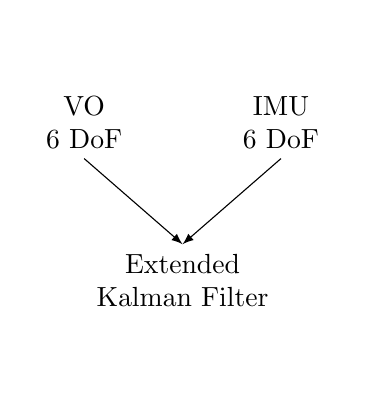
\begin{tikzpicture}[node distance=2.5cm, auto]
  \node[background] at (1.3,-1) {};
  \node [blockS] (s1) {\normalsize{VO\\6~DoF}};
  \node [blockS, right of=s1] (s2) {\normalsize{IMU\\6~DoF}};
  \node [blockS, below of=s1, xshift=1.25cm, node distance=2.0cm, text width=3cm] (s3) {\normalsize{Extended Kalman Filter}};

  \draw [arrow] (s1.south) to (s3.north);
  \draw [arrow] (s2.south) to (s3.north);
\end{tikzpicture}
